\section{Reinforcement Learning Training Details}
\label{appendix:rl_training}

\noindent\textit{This appendix covers training details for simulation-trained online RL
controllers (PPO, TD3, SAC, TQC, TRPO). World-model-based RL
(PPO-WM) is covered in Appendix~\ref{appendix:world_model};
MPPI is covered in Appendix~\ref{appendix:mppi_tuning};
offline RL (IQL) is covered in Appendix~\ref{appendix:offline_rl} below.}

\subsection{Algorithm and Architecture}

The RL controller uses Proximal Policy Optimization
(PPO)~\cite{schulman2017proximal} implemented via
StableBaselines3~\cite{stable_baselines3}.
The policy is parameterized by a two-layer MLP (\texttt{MlpPolicy},
$[64, 64]$ hidden units, \texttt{tanh} activations), consistent with the
SB3 default architecture.
A separate critic network of identical topology shares no weights with
the actor.
Table~\ref{tab:ppo_hyperparams} lists all hyperparameters; parameters
not shown retain SB3 library defaults.

\begin{table}[!t]
\centering
\renewcommand{\arraystretch}{1.15}
\caption{PPO Hyperparameters Used for Training}
\label{tab:ppo_hyperparams}
\begin{tabular}{lcc}
\toprule
\textbf{Parameter} & \textbf{Value} & \textbf{Source} \\
\midrule
Policy architecture                   & MlpPolicy {[}64, 64{]} & SB3 default \\
Activation function                   & \texttt{tanh}          & SB3 default \\
Total timesteps                       & 3\,000\,000            & configured  \\
Parallel environments                 & 16                     & configured  \\
Steps per rollout ($n_\text{steps}$)  & 2048                   & SB3 default \\
Mini-batch size                       & 64                     & SB3 default \\
Epochs per update                     & 10                     & SB3 default \\
Learning rate                         & $3\times10^{-4}$       & SB3 default \\
Discount factor $\gamma$              & 0.99                   & SB3 default \\
GAE $\lambda$~\cite{schulman2016gae}                         & 0.95                   & SB3 default \\
PPO clip range $\epsilon$             & 0.2                    & SB3 default \\
Entropy coefficient                   & 0.01                   & overridden  \\
Value function coefficient            & 0.5                    & SB3 default \\
Max gradient norm                     & 0.5                    & SB3 default \\
Device                                & CPU                    & configured  \\
\bottomrule
\end{tabular}
\end{table}

\subsection{Reward Function}
\label{appendix:reward_function}

We use a composite \emph{balanced} reward that combines position accuracy,
velocity damping, control effort, and jerk penalization:
\begin{equation}
\label{eq:reward}
\begin{aligned}
r_t = \operatorname{clip}\Big(\, & w_p\, r_\text{pos} - w_v\, p_\text{vel}
      - w_e \min(u_t^2, 1) \\
      & - w_j \min\big((u_t - u_{t-1})^2, 1\big)
      - p_\text{bnd},\; -1,\; 1 \Big)
\end{aligned}
\end{equation}
where
\begin{align*}
r_\text{pos} &= 0.6\,\exp\!\left(-\frac{\theta_t^2}{2\sigma_\text{out}^2}\right)
             + 0.4\,\exp\!\left(-\frac{\theta_t^2}{2\sigma_\text{in}^2}\right), \\
p_\text{vel} &= g_\theta \cdot \min\!\left(\frac{\dot\theta_t^2}{v_\text{max}^2},\; 1\right), \quad
  g_\theta = \exp\!\left(-\frac{\theta_t^2}{2\sigma_\text{gate}^2}\right), \\
p_\text{bnd} &= w_b\, \phi\!\left(\frac{|\theta_t|}{\theta_\text{max}}\right)
             + w_c\, \phi\!\left(\frac{|x_t|}{x_\text{max}}\right)\,
             \mathbf{1}[u_t\ \text{pushes into wall}], \\
  \phi(\rho) &= \left(\max\!\Big(0,\; \tfrac{\rho - 0.85}{0.15}\Big)\right)^{\!2},
\end{align*}
with $\sigma_\text{out} = \theta_\text{max}/4$, $\sigma_\text{in} = \theta_\text{max}/25$,
$\sigma_\text{gate} = \theta_\text{max}/10$, $v_\text{max} = 2$\,rad/s.
Weights are $w_p{=}0.60$, $w_v{=}0.25$, $w_e{=}0.05$, $w_j{=}0.05$,
$w_b{=}0.35$ (ball boundary), $w_c{=}0.20$ (cart wall). The cart-wall term
$w_c\,\phi(\cdot)$ applies only when the commanded action pushes the cart
further into the rail. The theoretical episode maximum is
$\approx 360$ (600 steps $\times$ 0.6/step).

\subsection{Training Environment}
\label{appendix:training_env}

We train the agent entirely in simulation using the full nonlinear
dynamics (Appendix~\ref{appendix:dynamics}), following established practices in
learning-based control~\cite{hewing2020learning}, integrated with a fourth-order
Runge--Kutta solver at the hardware control rate $\tau = 0.05$\,s (20\,Hz).
Sixteen parallel environments provide decorrelated rollout experience.
Episodes are time-limited to 600 steps (30\,s) via a gymnasium
\texttt{TimeLimit} wrapper. The environment itself does \emph{not}
terminate on cart-position or ball-angle limits: the \texttt{step}()
function always returns \texttt{terminated=False, truncated=False}, so the
only way an episode ends before 600 steps is the \texttt{TimeLimit}. In
particular, getting stuck at a wall (cart at the rail limit with the
ball still on the arc) does \emph{not} end the episode: the agent is
left to attempt recovery from the wall-stuck state, since this is a
realistic and frequent hardware scenario. Cart and ball excursions are
still penalized through the reward described below, but they are not
hard termination conditions.

The simulation incorporates key hardware characteristics:
\begin{itemize}
  \item \textbf{Motor model:} Two motor models appear in this study.
    A simplified first-order-lag model ($\tau_v{=}0.15$\,s, identified
    empirically, one-step command delay) is used for all five reported RL
    agents in Table~II (main paper), including PPO~(BZ+DR), and for the
    extended-training ablation. An S-curve profile (jerk-limited,
    $j_\text{max}{=}50\,\text{m/s}^3$, $a_\text{max}{=}15\,\text{m/s}^2$)
    that mirrors the drive's internal profiler is the development regime
    used elsewhere in this supplement. Appendix~\ref{appendix:rl_fairness}
    relates the two and confirms the choice does not affect the ranking.
  \item \textbf{Ball sensor staleness:} The ToF distance sensor updates at
    $\sim$10\,Hz while the control loop runs at 20\,Hz. Ball observations are
    held stale for a geometrically-distributed number of steps
    (mean~$= 2$ steps).
  \item \textbf{Domain randomization (DR):} At each episode reset,
    physical parameters (gravity, arc radius, friction coefficients,
    velocity lag $\tau_v$, dip geometry) are sampled uniformly
    from ranges centered on measured values.
\end{itemize}

\subsection{Training Curves}
\label{appendix:training_curves}

Figure~\ref{fig:training_curves} shows the evaluation reward during
training for all RL algorithms.  The off-policy methods (TD3, SAC, TQC)
reach their reward plateau early, within a fraction of their 1M-step
budget, whereas the PPO variants climb more gradually over a longer
schedule and cross the deployment-reward threshold only later in training.
Domain randomization generally reduces final reward
(the policy must succeed across a wider parameter distribution)
but improves hardware transfer.

\begin{figure}[!t]
  \centering
  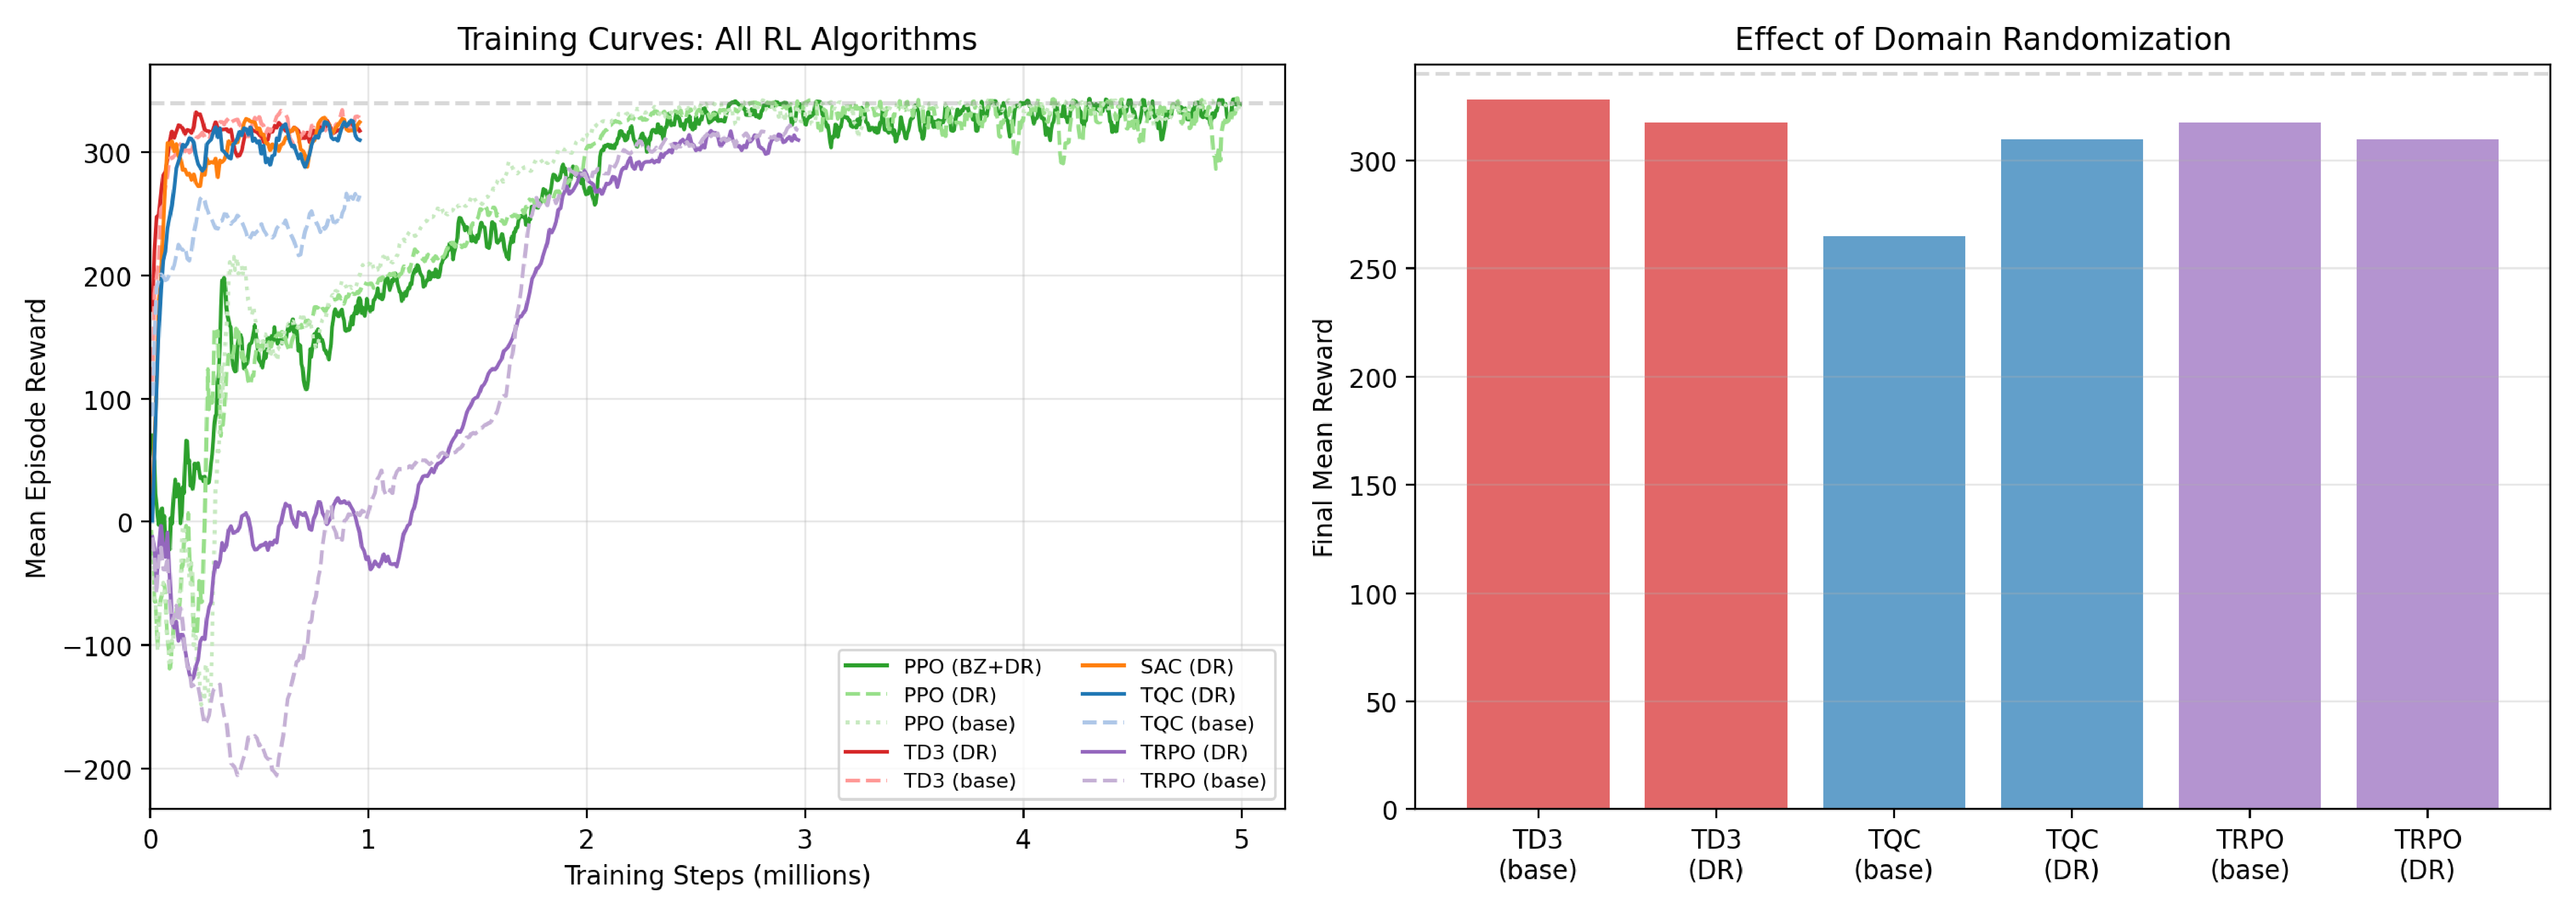
\includegraphics[width=\columnwidth]{figures/training_curves_all.eps}
  \caption{Left: Training curves (mean eval reward vs.~steps) for all
    RL algorithms.  Right: Effect of domain randomization on final
    reward.  DR slightly reduces sim performance but improves
    real-world success (see Appendix~\ref{appendix:multi_algo_hw}).}
  \label{fig:training_curves}
\end{figure}

\subsection{PPO Ablation Study}
\label{appendix:ppo_ablation}

We conducted a systematic ablation to identify which training
configuration factors most influence sim-to-real transfer quality.
We trained several PPO variants (3M steps each, S-curve motor,
seed~$=1$) and evaluated them on the same 50-trial stratified
initial-condition sequence used for the benchmark
(Section~\ref{sec:ic_design}). The ablation factors are the reward
function (balanced vs.~Gaussian), domain randomization (DR), and the
blind-zone sensor model (BZ); their combinations are listed in
Table~\ref{tab:ppo_ablation}.

All variants used the S-curve motor model and ball sensor staleness.

\subsubsection{Results}

Table~\ref{tab:ppo_ablation} reports the best checkpoint per variant
(selected by highest success rate, then fastest settling) evaluated
with 50 stratified trials, settling band $= 0.01$\,rad,
settling duration $= 1.0$\,s.

\begin{table*}[!t]
\centering
\renewcommand{\arraystretch}{1.15}
\caption{PPO ablation study: simulation (S-curve motor model). Every row
  except Gaussian is a 50-trial stratified evaluation from
  \texttt{rl\_ablation/blind\_zone\_ablation.json}; the Gaussian row is a
  20-trial checkpoint screen (seed 42) from
  \texttt{rl\_ablation/ppo\_checkpoint\_sweep.json}. ``Settle'' is the mean
  over successful trials; ``RMS Effort'' is the RMS commanded action
  averaged over trials (the Gaussian value is derived from the stored
  squared effort).}
\label{tab:ppo_ablation}
\begin{tabular}{lcccc}
\toprule
\textbf{Variant} & \textbf{Ckpt} & \textbf{SR} & \textbf{Settle (s)}
  & \textbf{RMS Effort} \\
\midrule
Balanced          & best  & 100\% & 1.72 & 0.078 \\
Gaussian          & final &  95\% & 2.22 & 0.731 \\
Balanced + BZ     & best  &  96\% & 2.37 & 0.145 \\
Balanced + BZ + DR& best  & 100\% & 1.67 & 0.096 \\
Balanced + DR     & final & 100\% & 1.49 & 0.076 \\
\bottomrule
\end{tabular}
\end{table*}

\subsubsection{Analysis}

\paragraph{Reward function.}
The composite \emph{balanced} reward achieves 100\% simulation
success with far lower control effort than the pure-Gaussian
reward (RMS effort 0.078 vs.\ 0.731). The Gaussian reward lacks
explicit effort and jerk penalties; its hardware validation
(Table~\ref{tab:ppo_hardware}, 30\% SR / 15.62\,s over 10 trials)
confirms that the oscillatory behavior translates directly to
real-world failure.

\paragraph{Blind-zone and domain randomization.}
Adding the blind-zone model alone (Balanced+BZ) drops simulation
SR slightly (96\%), consistent with the policy overfitting to a fixed
blind-zone threshold. Adding DR on top (Balanced+BZ+DR) recovers 100\%
simulation SR (1.67\,s); DR randomizes the blind-zone threshold together
with the physical and observation-noise parameters, so the recovery is not
attributable to threshold randomization alone. This is the configuration behind PPO~(BZ+DR). Its S-curve
policy reaches 98\% hardware SR over 50 trials, while the matched
first-order-lag checkpoint reported in Table~II (main paper) reaches 96\%
(Appendix~\ref{appendix:rl_fairness}).
DR alone (Balanced+DR) also reaches 100\% simulation SR with the
lowest control effort (0.076).

\paragraph{Training duration.}
Figure~\ref{fig:ppo_checkpoints} shows that 1--1.5M steps is the
best trade-off: at 500K steps all variants achieve $\leq 85$\% SR;
beyond $\sim$2M steps settling time increases as the policy becomes
more conservative without improving reliability.

\begin{figure}[!t]
  \centering
  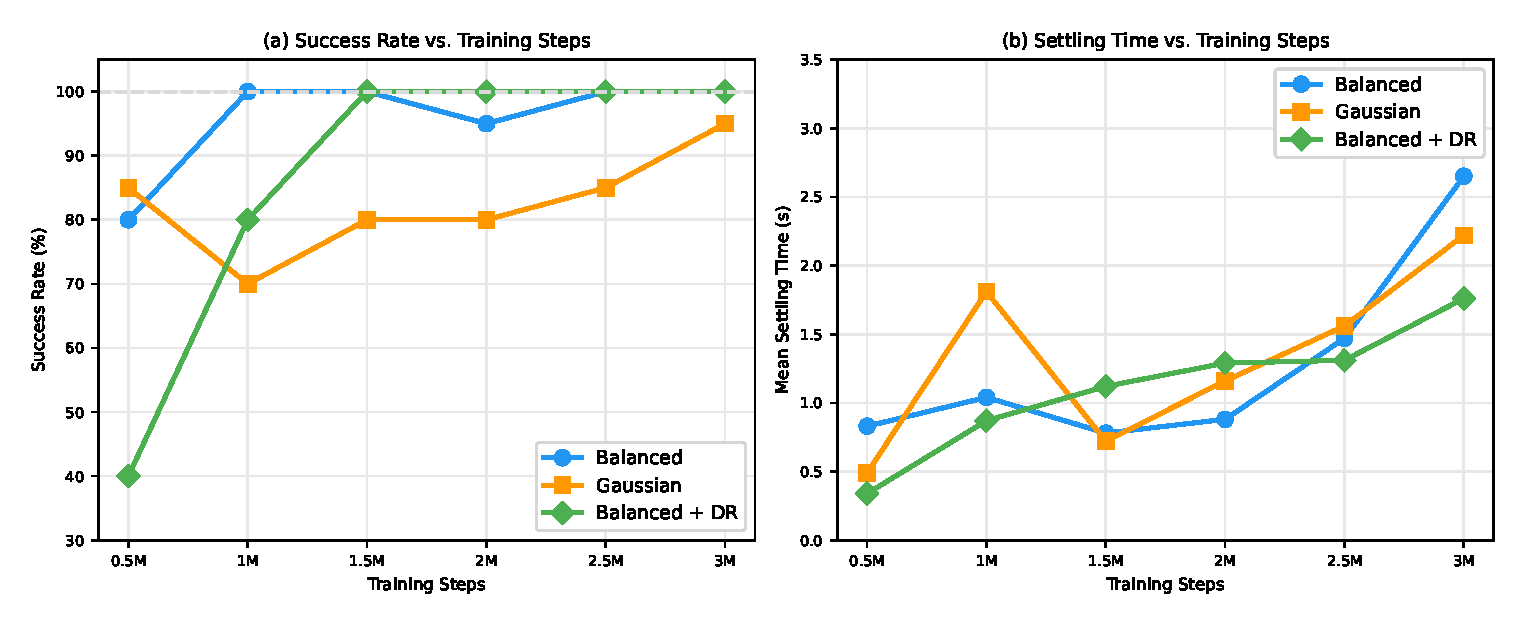
\includegraphics[width=0.99\columnwidth]{figures/ppo_ablation_checkpoints.eps}
  \caption{Success rate and mean settling time vs.~training
    checkpoint for the PPO variants.
    Balanced and Balanced+DR reach 100\% SR by 1--1.5M steps;
    Gaussian plateaus below 100\%.}
  \label{fig:ppo_checkpoints}
\end{figure}

\subsection{Hardware Validation of PPO Variants}
\label{appendix:ppo_hardware}

To validate the simulation ablation findings, we tested the top three PPO
variants on real hardware (10 trials each, stratified
initial conditions, identical protocol to Section~\ref{sec:ic_design}).

\begin{table*}[!t]
\centering
\renewcommand{\arraystretch}{1.15}
\caption{PPO hardware validation (10 trials per variant).}
\label{tab:ppo_hardware}
\begin{tabular}{lccc}
\toprule
\textbf{Variant} & \textbf{SR} & \textbf{Settle (s)}
  & \textbf{Max (s)} \\
\midrule
Balanced (no DR) & 100\% & 5.26 & 15.81 \\
Balanced + DR    & 100\% & 6.94 & 21.66 \\
Gaussian         &  30\% & 15.62 & 28.11 \\
\bottomrule
\end{tabular}
\end{table*}

\subsubsection{Hardware Insights}

\paragraph{Reward function on hardware.}
The Gaussian-reward policy fails 70\% of hardware trials, confirming
that the aggressive oscillatory behavior observed in simulation
translates directly to real-world failure.
The composite \emph{balanced} reward's effort and jerk penalties
produce smooth, hardware-compatible control signals.

\paragraph{Sim-to-real settling gap.}
Hardware settling times are 3--5$\times$ slower than simulation
(sim: 1.5--1.7\,s $\to$ hw: 5.3--6.9\,s).
The simulation-to-hardware characterization in
Appendix~\ref{appendix:simulation_validation} identifies plausible
contributors to this gap: sensor characteristics (the $\sim$82\,ms ToF cycle
and the $|\theta|>0.071$\,rad saturation) and the higher-order motor
response (the S-curve profile approximated as first-order lag); ball-arc
friction and the uncontrolled initial ball velocity likely add further
variance. This is inferred from the open-loop prediction analysis rather
than a controlled controller-level ablation.

\paragraph{Domain randomization: sim-to-real trade-off.}
Both balanced variants achieve 100\% hardware success rate.
In simulation, DR is \emph{faster} (1.49 vs.\ 1.72\,s) due to
its regularization effect.
On hardware, this inverts: the no-DR model settles 24\% faster
(5.26 vs.\ 6.94\,s), consistent with the real system being close to the
nominal parameters it was trained on.
The DR model's policy is smoother but more cautious on the
real system.
For long-term deployment where hardware properties may drift
(mechanical wear, temperature drift), DR is plausibly the more robust
choice, though we did not run a drift experiment to confirm this.

\subsection{Multi-Algorithm Comparison}
\label{appendix:multi_algo}

We trained five RL algorithms with the \emph{balanced} reward, each
in two variants (base: nominal dynamics; DR: domain randomization).
On-policy algorithms (PPO, TRPO~\cite{schulman2015trpo}) used 16 parallel
environments; off-policy algorithms (SAC~\cite{haarnoja2018sac},
TD3~\cite{fujimoto2018td3}, TQC~\cite{kuznetsov2020controlling})
used 1 environment.
PPO and TRPO use two-layer MLPs with $[64,64]$ hidden units; SAC and TQC use
the Stable-Baselines3 default of $[256,256]$, and TD3 uses its default of
$[400,300]$. Each algorithm therefore keeps its library
default rather than a hand-tuned network. All five algorithms were trained
with the same single seed (seed~1) under the deterministic Hydra
configuration (\texttt{training/configs/train.yaml}), so cross-algorithm
differences are not confounded by seed choice; per-algorithm
training-stochasticity variance is not characterized.
Table~\ref{tab:rl_training_cost} summarizes the training cost;
Table~\ref{tab:rl_comparison} reports simulation evaluation.

\paragraph{Model selection.}
For each training run, all saved checkpoints are evaluated through
simulation (50 trials, stratified ICs). Three models are selected
for hardware deployment: (1)~the checkpoint with the highest
simulation success rate, (2)~the final checkpoint at the end of
training, and (3)~an intermediate checkpoint that achieves good
performance without being the absolute best or final (to capture
potential overfitting). The model that performs best on hardware
is reported in the main results. SB3's \texttt{EvalCallback}
(10 deterministic episodes every 50K steps) is used only for
training progress monitoring, not for final model selection.

\begin{table*}[!t]
\centering
\renewcommand{\arraystretch}{1.15}
\caption{Training cost per algorithm (Intel i5, CPU only).}
\label{tab:rl_training_cost}
\begin{tabular}{lccccc}
\toprule
\textbf{Algorithm} & \textbf{Type} & \textbf{$n_\text{envs}$}
  & \textbf{Steps} & \textbf{Wall-clock} & \textbf{$\geq$300 step} \\
\midrule
PPO   & on-policy  & 16 & 3.0M & $\sim$40\,min   & 1.35--2.0M \\
TRPO  & on-policy  & 16 & 3.0M & $\sim$58\,min   & 1.0--1.35M \\
SAC   & off-policy &  1 & 1.0M & $\sim$5.7\,h    & 150--250K \\
TD3   & off-policy &  1 & 1.0M & $\sim$5.7\,h    & 50--250K \\
TQC   & off-policy &  1 & 1.0M & $\sim$8.5\,h  & 100--200K \\
\bottomrule
\end{tabular}
\end{table*}

\noindent
The ``$\geq$300 step'' column indicates the first training step at which
the evaluation reward exceeded 300 (a functional policy threshold;
theoretical maximum is 360 for 600 steps).
On-policy methods are faster in wall-clock time due to 16-environment
parallelism despite requiring more total environment steps.
Among the off-policy methods (single environment), TD3 reaches the
functional-policy threshold in the fewest steps (from about 50K), while
TQC has the longest wall-clock time (about 8.5\,h).

\begin{table*}[!t]
\centering
\renewcommand{\arraystretch}{1.15}
\caption{Multi-algorithm comparison: simulation (50 trials, first-order motor model)
  and hardware (50 stratified trials) success rate and settling time.
  Sim settling is computed over successful trials; hardware SR ranges from 60--96\%.}
\label{tab:rl_comparison}
\begin{tabular}{lccccc}
\toprule
\textbf{Model} & \textbf{SR} & \textbf{Sim Mean (s)} & \textbf{Med.\,(s)}
  & \textbf{HW SR} & \textbf{HW Mean (s)} \\
\midrule
PPO (base)  & 100\% & 1.72 & 1.25 & 60\%  & 3.53 \\
PPO (BZ+DR) &  96\% & 0.82 & 0.40 & 96\%  & 3.81 \\
SAC (DR)    & 100\% & 0.98 & 0.60 & 82\%  & 10.10 \\
TD3 (DR)    & 100\% & 1.78 & 0.55 & 92\%  & 11.45 \\
TQC (DR)    & 100\% & 1.89 & 0.60 & 86\%  & 9.77 \\
TRPO (DR)   & 100\% & 3.88 & 2.18 & 90\%  & 8.09 \\
\bottomrule
\end{tabular}
\end{table*}

\subsubsection{Algorithm Analysis}

The simulation settling times in Table~\ref{tab:rl_comparison} are those of
the \emph{deployed} checkpoints (the same policies as in
Table~\ref{tab:full_results}), reproduced on the shipped models. The
blind-zone and domain-randomization ablations later in this appendix instead
report the S-curve development family (Appendix~\ref{appendix:rl_fairness}),
whose simulation settling differs accordingly; the two should not be compared
directly.

\paragraph{PPO and SAC settling time.}
At their deployed checkpoints, PPO~(BZ+DR) has the fastest simulation
settling (0.82\,s) among these configurations, at 96\% SR; SAC~(DR)
reaches 100\% SR and settles in 0.98\,s mean (0.60\,s
median). PPO also has lower control effort. The 16-environment
parallelism makes PPO the most wall-clock efficient (40\,min vs.\
90+\,min for SAC).

\paragraph{SAC with DR and longer training.}
At its deployed checkpoint SAC~(DR) settles in 0.98\,s (simulation) at
100\% SR. SAC reaches a functional policy (reward $\geq 300$) in about
150K steps (Table~\ref{tab:rl_training_cost}), fewer than PPO, and both
domain randomization and longer training improve settling relative to
shorter runs.

\paragraph{TD3 across training budgets.}
At its deployed checkpoint TD3~(DR) settles in 1.78\,s (simulation) at
100\% SR, and longer training improves settling over shorter budgets.
TD3~(DR) converges fastest of all algorithms
(reward $\geq 300$ at 50K steps, Table~\ref{tab:rl_training_cost}).

\paragraph{TQC across training budgets.}
At its deployed checkpoint TQC~(DR) reaches 100\% SR with 1.89\,s mean
settling (simulation). Its truncated quantile critics (25 atoms per
critic) require more training budget than SAC or TD3 to reach strong
performance, but converge to a reliable policy given enough training.

\paragraph{TRPO and DR.}
At 3M steps, the deployed TRPO~(DR) checkpoint reaches 100\% simulation
SR with 3.88\,s mean settling, the slowest of the DR agents.
TRPO~(base) drops to 90\% SR with longer training,
suggesting overfitting to nominal dynamics.
The conservative trust-region updates produce smooth control
(ISE$_u \approx 0.03$) but cannot match PPO/SAC speed.

\subsubsection{Failure Mode Analysis}

Across the seven simulation-trained RL controllers evaluated with 50
hardware trials each (350 trials total), the dominant predictor of failure is
the training configuration, not the initial-condition stratum
(Tables~\ref{tab:full_results} and~\ref{tab:failed_variants}), and the stratum pattern that does appear runs
opposite to the expectation that the most constrained starts are the
hardest:

\paragraph{Blind-zone modeling and DR.}
The base PPO policy (no DR, no BZ) fails on 20/50 trials (60\% SR);
adding DR reduces this to 5/50 (PPO~(DR), 90\%), and adding both DR
and the blind-zone model reduces it to a single failure
(PPO~(BZ+DR), 98\% in the S-curve training family;
Appendix~\ref{appendix:rl_fairness}). SAC~(DR)
(82\%, 9 failures) and TQC~(DR) (86\%, 7 failures), which are not
trained with the blind-zone model, fail more often than PPO~(BZ+DR),
consistent with the blind-zone being a contributing cause of RL
hardware failures.

\paragraph{Failure distribution across strata.}
Contrary to the expectation that the most constrained starts are the hardest,
the failures spread across strata, and the at-wall-opposite start is among the
easiest rather than the hardest. The center and mid-rail starts draw as many
failures as the constrained ones or more: the single PPO~(BZ+DR) failure of the
S-curve development checkpoint is on a center start (cart at $-0.09$\,m), not at
a wall (the deployed first-order-lag checkpoint of Table~\ref{tab:full_results}
instead misses two at-wall-same trials), and TD3 and TRPO also miss on center. This echoes the pattern that the center and
mid-rail starts, despite offering the most maneuvering room, are where these
RL controllers fail most: with the cart already positioned and no wall to use
as a momentum backstop, the controller must wait out the ball's own dynamics.

\subsubsection{Full Hardware Evaluation (50 Trials)}
\label{appendix:multi_algo_hw}

Every model-free RL algorithm (the DR variant of each off-policy method,
together with PPO~(BZ+DR)) was evaluated on hardware over the full 50
stratified trials (same protocol as Section~\ref{sec:ic_design}).

\begin{table*}[!t]
\centering
\renewcommand{\arraystretch}{1.15}
\caption{Full hardware evaluation: RL models (50 trials each,
         stratified ICs).}
\label{tab:rl_hw_50trial}
\begin{tabular}{lccccc}
\toprule
\textbf{Model} & \textbf{HW SR} & \textbf{Settle (s)}
  & \textbf{Med (s)} & \textbf{Max (s)} & \textbf{Sim SR} \\
\midrule
PPO (BZ+DR) & 96\% & 3.81 & 3.15 & 13.90 & 96\% \\
TD3 (DR)    & 92\% & 11.45 & 10.06 & 28.11 & 100\% \\
TRPO (DR)   & 90\% & 8.09 & 4.80 & --  & 100\% \\
PPO (DR)    & 90\% & 5.11 & 2.55 & 22.85 & 100\% \\
TQC (DR)    & 86\% & 9.77 & 6.61 & --  & 100\% \\
SAC (DR)    & 82\% & 10.10 & 8.40 & --  & 100\% \\
PPO (base)  & 60\% & 3.53 & 2.53 & 10.55 & 100\%  \\
\bottomrule
\end{tabular}
\end{table*}

\paragraph{50-trial results.}
Over the full 50-trial evaluation (Table~II, main paper),
PPO~(BZ+DR) achieves 96\% SR, with two failures on at-wall-same trials.
PPO~(DR) achieves 90\% SR. In the matched S-curve development ablation,
adding the blind-zone model lifts PPO~(BZ+DR) from 90\% to 98\%
(+8 percentage points); the deployed first-order-lag checkpoint of
Table~II reaches 96\%.
PPO~(base) at 60\% indicates that domain randomization is important
for sim-to-real transfer at this training budget (single training seed).

\subsection{Extended Training: 5M-Step Ablation}

While the main 3M-step ablation shows that blind-zone modeling is
the efficient path to high hardware SR, we also evaluated PPO
variants at extended timesteps on hardware (50 trials each,
Table~\ref{tab:ppo_5m_hw}):

\begin{table}[H]
\centering
\caption{PPO 5M-step hardware evaluation (50 trials, 20\,Hz).}
\label{tab:ppo_5m_hw}
\begin{tabular}{lccc}
\toprule
\textbf{Variant} & \textbf{Steps} & \textbf{HW SR} & \textbf{Median (s)} \\
\midrule
PPO base (no DR, no BZ)  & 5.0M  & 100\% & 3.05 \\
PPO BZ+DR                & 2.75M & 96\%  & 3.15 \\
PPO BZ+DR                & 3.50M & 94\%  & 3.30 \\
PPO DR                    & 2.25M & 84\%  & 4.55 \\
\bottomrule
\end{tabular}
\end{table}

Base PPO at 5M steps (first-order motor model) achieves 100\% SR with no
domain randomization and no blind-zone modeling, above the 3M base
variant (60\%). This suggests extended training can partly compensate for
missing sensor awareness, though the two baselines differ in motor regime
(first-order vs.\ S-curve development) and each is a single checkpoint, so
the comparison is not fully controlled.
However, PPO~(BZ+DR) at 3M steps remains the more time-efficient
approach (98\% SR in $\sim$40\,min vs.\ 100\% SR in $\sim$67\,min).
BZ+DR performance is slightly lower at 3.5M steps (94\%). PPO~(DR) at
2.25M steps underperforms the 3M DR variant (84\% vs.\ 90\%). These are
single-checkpoint point estimates, so we report them as observations rather
than controlled trends.

\noindent In these runs, sensor modeling (BZ) and extended training
each improved the observed sim-to-real transfer. BZ
offers training efficiency (98\% at 3M), while extended training
reaches higher reliability (100\% at 5M) at the cost of longer
training time.

\paragraph{Simulation vs hardware ranking.}
SAC~(DR) reaches 100\% simulation SR but only 82\% hardware SR over
50 trials, the most aggressive sim-to-real gap among the RL controllers
that still achieve 100\% simulation SR, suggesting its policy exploits
simulation dynamics that do not transfer.
TRPO's conservative trust-region updates leave it too cautious to
recover from some real perturbations within the 30\,s time limit;
it nonetheless reaches 90\% SR over 50 trials.

\paragraph{TD3 and longer training.}
The deployed TD3~(DR) checkpoint (1M steps) reaches 92\% SR over the
full 50-trial evaluation. TD3 transfers to hardware better than SAC
but still cannot match PPO's robustness.

\paragraph{Overall ranking.}
PPO's on-policy training with 16 parallel environments produces
policies that generalize to hardware most reliably.
The combination of PPO + DR + blind-zone modeling achieves
96\% SR over 50 hardware trials with 3.81\,s mean settling (the
first-order-lag checkpoint of Table~II, main paper).
No off-policy algorithm matches this: TD3~(DR) is closest
at 92\% SR but with about three times the settling time (11.45\,s).

\subsection{Sensor Blind Zone Ablation}
\label{appendix:blind_zone}

The VL53L0X sensor exhibits a minimum-range blind-zone
(Appendix~\ref{appendix:sensor_characterization}): when the ball
is within $\sim$40\,mm of a sensor ($|\theta| > 0.071$\,rad),
the reading saturates and the controller observes the ball
``stuck'' at the boundary.
We introduced an optional blind-zone model in the training
environment (Appendix~\ref{appendix:sensor_sim_model}) and trained two
additional PPO variants: one with blind-zone only (BZ), one with
both blind-zone and domain randomization (BZ+DR).

\begin{table*}[!t]
\centering
\renewcommand{\arraystretch}{1.15}
\caption{Blind zone ablation: simulation evaluation
         (50 trials, evaluated \emph{without} blind-zone to isolate
         control quality).}
\label{tab:blind_zone_sim}
\begin{tabular}{lccccc}
\toprule
\textbf{Training Config} & \textbf{BZ} & \textbf{DR}
  & \textbf{SR} & \textbf{Settle (s)} \\
\midrule
Balanced          & No    & No    & 100\% & 1.72 \\
Balanced + DR     & No    & Yes & 100\% & 1.49 \\
Balanced + BZ     & Yes & No    &  96\% & 2.37 \\
Balanced + BZ+DR  & Yes & Yes & 100\% & 1.67 \\
\bottomrule
\end{tabular}
\end{table*}

\begin{table*}[!t]
\centering
\renewcommand{\arraystretch}{1.15}
\caption{Blind zone ablation: hardware validation (10 trials each).}
\label{tab:blind_zone_hw}
\begin{tabular}{lccccc}
\toprule
\textbf{Training Config} & \textbf{BZ} & \textbf{DR}
  & \textbf{SR} & \textbf{Settle (s)} & \textbf{Max (s)} \\
\midrule
Balanced          & No    & No    & 100\% & 5.26 & 15.81 \\
Balanced + DR     & No    & Yes & 100\% & 6.94 & 21.66 \\
Balanced + BZ     & Yes & No    &  60\% & 2.72 &  9.46 \\
Balanced + BZ+DR  & Yes & Yes & 100\% & 4.98 & 13.66 \\
\bottomrule
\end{tabular}
\end{table*}

\paragraph{Blind-zone model and DR.}
Without DR, the blind-zone model makes training harder (96\% sim SR,
60\% hardware SR): the policy overfits to a fixed blind-zone
threshold and cannot generalize to the real sensor's variable
minimum range.
With DR (which randomizes the threshold over
$[0.060, 0.080]$\,rad), the policy achieves 100\% hardware SR
and settles 28\% faster than the previous best (4.98 vs.\ 6.94\,s).

\paragraph{Sim-to-real gap.}
The settling-time ratio (hardware/sim) improves from
$4.7\times$ (no BZ: $6.94/1.49$) to $3.0\times$ (BZ+DR:
$4.98/1.67$), consistent with the blind-zone model
capturing part of the sim-to-real gap (single training seed).

\subsection{Complete Ablation Summary}
\label{appendix:ablation_summary}

Table~\ref{tab:full_ablation} consolidates all PPO ablation
variants with both simulation and hardware results, and
Fig.~\ref{fig:ppo_ablation_summary} shows the same comparison visually: the
Balanced+BZ+DR variant achieves the best combined performance, 100\% hardware
SR at the lowest sim-to-real settling gap (3.0$\times$).

\begin{table*}[!t]
\centering
\renewcommand{\arraystretch}{1.15}
\caption{Complete PPO ablation: simulation (50 trials, except the
         Gaussian-wall row, a 20-trial checkpoint screen) and
         hardware (10 trials). All variants trained for 3M steps
         with balanced reward unless noted.}
\label{tab:full_ablation}
\begin{tabular}{lcc|cc}
\toprule
 & \multicolumn{2}{c|}{\textbf{Simulation}} & \multicolumn{2}{c}{\textbf{Hardware}} \\
\textbf{Variant} & \textbf{SR} & \textbf{Settle} & \textbf{SR} & \textbf{Settle} \\
\midrule
Balanced (base)         & 100\% & 1.72\,s & 100\% & 5.26\,s \\
Balanced + DR           & 100\% & 1.49\,s & 100\% & 6.94\,s \\
Gaussian                &  95\% & 2.22\,s &  30\% & 15.62\,s \\
Balanced + BZ           &  96\% & 2.37\,s &  60\% &  2.72\,s \\
\textbf{Balanced + BZ+DR} & \textbf{100\%} & \textbf{1.67\,s} & \textbf{100\%} & \textbf{4.98\,s} \\
\bottomrule
\end{tabular}
\end{table*}

\begin{figure}[!t]
  \centering
  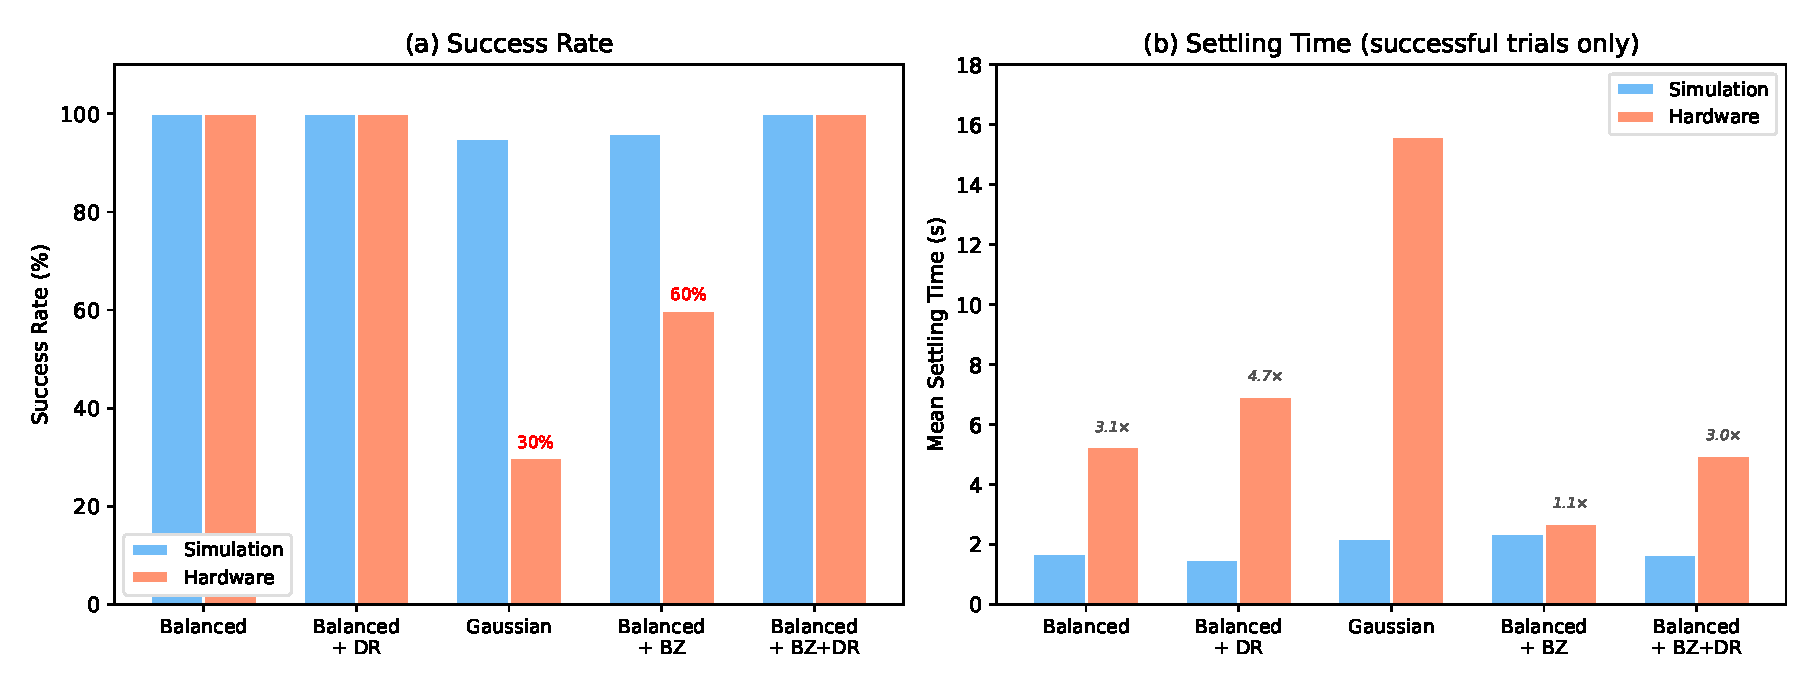
\includegraphics[width=0.99\columnwidth]{figures/ppo_ablation_summary.eps}
  \caption{Complete PPO ablation summary: success rate (a) and mean
    settling time (b) across simulation and hardware.
    Annotations in (b) show the sim-to-real settling ratio.
    The Balanced+BZ+DR variant achieves the best combined
    performance: 100\% hardware SR with the lowest sim-to-real gap
    (3.0$\times$).}
  \label{fig:ppo_ablation_summary}
\end{figure}

\subsection{Selected Model}
\label{appendix:selected_model}

Based on the complete ablation (Table~\ref{tab:full_ablation}), the
deployed PPO controller (Table~II in the main paper, reported as
PPO~(BZ+DR)) uses:
\begin{itemize}
  \item \textbf{Motor model:} The PPO~(BZ+DR) reported in Table~II of the
        main paper is the matched first-order-lag checkpoint, the same
        model used for the other four RL agents
        (Appendix~\ref{appendix:rl_fairness}). The S-curve profile
        (jerk-limited, mirroring the drive's internal profiler) was the
        development regime used for the ablations elsewhere in this
        supplement (Appendix~\ref{appendix:motor_fwhm_ablation},
        Table~\ref{tab:fwhm20_hw_10t}).
  \item Reward: \emph{balanced} (Eq.~\ref{eq:reward})
  \item Domain randomization: enabled
  \item Sensor blind-zone model: enabled
  \item Observation: standard 4-dimensional state
    $[x, \dot{x}, \theta, \dot{\theta}]$
  \item Training: extended sweep, best checkpoint at 2.75M steps
    (matched first-order-lag, Table~\ref{tab:ppo_5m_hw})
\end{itemize}

In simulation (50 trials): 100\% SR, mean settling 1.67\,s.
On hardware (50 trials), the matched first-order-lag checkpoint reported
in Table~II reaches 96\% SR, mean settling 3.81\,s (two failures); the
S-curve development policy reaches 98\%, 5.11\,s.

This configuration gives the highest hardware reliability among the
simulation-trained model-free RL controllers. In the development ablation, blind-zone modeling
lowers the sim-to-real settling gap from 4.7$\times$ (without it, $6.94/1.49$) to
3.0$\times$ ($4.98/1.67$).

\subsection{Motor Model and Dip-Width (FWHM) Ablation}
\label{appendix:motor_fwhm_ablation}

The original PPO models were trained with an S-curve motor profile
and a dip width of FWHM$= 42$\,mm in the simulation environment.
After independent measurement of the physical dip (FWHM$\approx 20$\,mm,
measured via sensor calibration), we conducted a systematic ablation
of these two training-environment parameters.

\subsubsection{Training configurations}

Two PPO training regimes were compared at FWHM$=20$\,mm:
\begin{enumerate}
  \item \textbf{FWHM=20, S-curve, 3M}: the original motor model,
    four sub-variants (base, DR, BZ+DR, Gaussian-wall).
  \item \textbf{FWHM=20, first-order, 5M}: the simplified
    first-order-lag motor model (no jerk/acceleration limits), trained
    for 5M steps, four sub-variants (base, DR, BZ+DR, Gaussian-wall).
\end{enumerate}

\subsubsection{Hardware screening (10 trials)}

Table~\ref{tab:fwhm20_hw_10t} reports the 10-trial hardware screening
for both regimes (data file: \texttt{rl\_finetuning/fwhm20\_ablation\_summary.json}).
This is a screening comparison, not the definitive 50-trial benchmark
of Table~II (main paper).

\begin{table*}[!t]
\centering
\renewcommand{\arraystretch}{1.15}
\caption{FWHM=20\,mm ablation, 10-trial hardware screening.
  SR and mean settling (successful trials) for S-curve-trained vs.
  first-order-trained PPO variants.}
\label{tab:fwhm20_hw_10t}
\begin{tabular}{lcccc cc}
\toprule
 & & \multicolumn{2}{c}{\textbf{S-curve trained}} & \multicolumn{2}{c}{\textbf{first-order trained}} \\
\cmidrule(lr){3-4}\cmidrule(lr){5-6}
\textbf{Variant} & & SR & Settle (s) & SR & Settle (s) \\
\midrule
PPO base          & & 100\% & 8.14 & 100\% & 11.06 \\
PPO +DR           & &  80\% & 6.33 &  90\% &  5.45 \\
PPO +BZ+DR        & &  90\% & 5.11 &  90\% &  6.58 \\
PPO Gaussian-wall & &  90\% & 6.14 &  80\% & 12.84 \\
\bottomrule
\end{tabular}
\end{table*}

\paragraph{FWHM=20\,mm vs.\ 42\,mm.}
On 10-trial screening the FWHM=20\,mm variants are competitive with
the deployed FWHM=42\,mm variants (whose S-curve 50-trial result is
PPO~(BZ+DR) 98\%/5.11\,s; Table~II (main paper) reports the matched
first-order-lag checkpoint at 96\%/3.81\,s). The dip-width
mismatch does not measurably degrade hardware performance at the 10-trial screening level (single training seed);
this is consistent with domain randomization varying the dip parameters
during training regardless of the nominal value.

\paragraph{First-order vs.\ S-curve training.}
Figure~\ref{fig:ppo_fo_5M_reward} shows the training-reward curves for
the three first-order 5M variants (eval reward, 20 deterministic episodes
every 5K steps; data files: \texttt{rl\_5m\_ablation/training\_runs/ppo\_fo\_5M\_*}).
All three converge to near-theoretical-maximum reward by ~2--3M steps and
remain stable through 5M, with the DR and BZ+DR variants reaching the
plateau slightly later than base. We report training-reward curves rather
than per-checkpoint hardware SR here because the per-checkpoint 50-trial
hardware evaluation of the first-order 5M checkpoints is not included in
this preprint; the deployed PPO~(BZ+DR) reported in Table~II (main paper) is the
matched first-order-lag checkpoint at 96\% SR; the S-curve
(3M, FWHM=42\,mm) policy reaches 98\% and is the development regime used
elsewhere in this supplement.

\begin{figure}[!t]
  \centering
  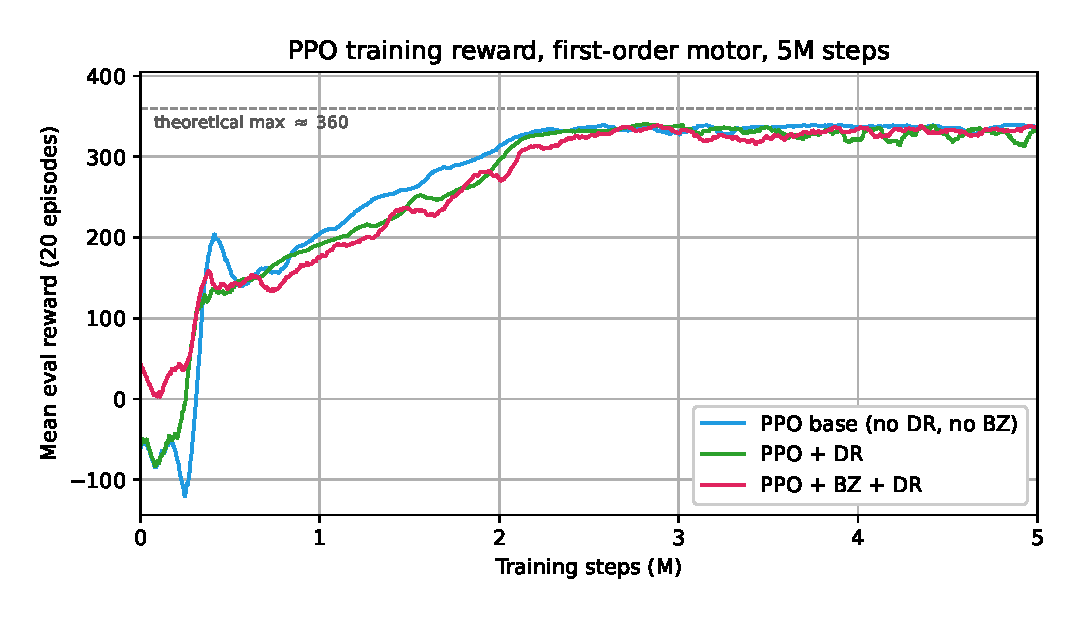
\includegraphics[width=\columnwidth]{figures/ppo_fo_5M_reward_curves.eps}
  \caption{First-order 5M PPO training-reward curves (mean eval reward
    vs.~training step, 20 episodes per checkpoint). Base, DR, and BZ+DR
    all plateau near the theoretical maximum (~360) by ~2--3M steps.
    }
  \label{fig:ppo_fo_5M_reward}
\end{figure}

\paragraph{FWHM mismatch.}
Training with FWHM$= 42$\,mm (2.1$\times$ the true value) does not
degrade hardware performance relative to the correct value.
This contrasts with NMPC, where the same conservative dip-width mismatch
materially helps hardware performance (Appendix~\ref{appendix:tuning_insights}).
For RL, the policy learns to handle the dip regardless of its
training-time width, provided domain randomization varies the dip
parameters during training.

\subsection{Fairness of the RL Comparison}
\label{appendix:rl_fairness}

The five simulation-trained RL agents in Table~II (main paper) are all
trained against the same first-order-lag motor model, but reaching that
consistency required a correction. An earlier PPO~(BZ+DR) policy used the
S-curve profile that mirrors the drive's internal profiler, whereas TD3,
SAC, TQC, and TRPO used the simplified first-order-lag approximation.
Because the S-curve is the closer match to the physical drive, that
asymmetry could in principle have flattered PPO.

To remove it, we re-trained PPO~(BZ+DR) under the same first-order-lag
model used for the other four agents and evaluated it over the identical
50-trial stratified protocol. The matched policy reaches 96\% hardware SR
(95\% CI $[87, 99]$, median settling 3.15\,s; best checkpoint of the
extended-training sweep, Table~\ref{tab:ppo_5m_hw}), and this is the
policy reported in Table~II. The earlier S-curve policy reaches 98\% and is
the one used elsewhere in this supplement, where the S-curve training
family is the consistent development regime: the fine-tuning study
(Appendix~\ref{appendix:finetuning}), the world-model comparison
(Appendix~\ref{appendix:world_model}), and the domain-randomization and
blind-zone ablations. Under either motor model PPO~(BZ+DR) remains the
most reliable and fastest-settling of the simulation-trained agents, so
the ranking and every qualitative finding are unchanged.

A second asymmetry concerns the blind-zone sensor model, added to PPO but
not to TD3, SAC, TQC, or TRPO. The off-policy agents take six to nine
hours each to train (Table~\ref{tab:rl_training_cost}), so the exhaustive
reward-and-sensor-model ablation that produced PPO~(BZ+DR) was practical
only for the on-policy PPO ($\sim$40\,min per run). We therefore read
PPO's lead as the strongest RL configuration we tested rather than
evidence that PPO is the best algorithm; the controlled claim, that
modeling the blind-zone helps, rests on the within-PPO ablation
(PPO~(DR) 90\% to PPO~(BZ+DR) 98\% in the matched S-curve ablation),
not on the cross-agent comparison.

\subsection{Simulation-to-Real Transfer}
\label{appendix:sim2real}

The trained policy is deployed on hardware without any online
fine-tuning or parameter adjustment (zero-shot transfer).
The primary sources of sim-to-real gap are:
\begin{enumerate}
  \item \textbf{Sensor blind-zone:} Near the arc boundaries
        ($|\theta| > 0.071$\,rad), the VL53L0X reports a saturated
        reading due to its minimum-range limitation
        ($\sim$30--50\,mm, Appendix~\ref{appendix:sensor_characterization}).
        The blind-zone model introduced in training reduces this gap
        from 4.7$\times$ to 3.0$\times$.
  \item \textbf{Sensor latency:} The ToF sensor cycle ($\sim$82\,ms)
        exceeds the control timestep (50\,ms), so the policy acts
        on ball-position measurements that may be one full
        sensor cycle old.
        This is modeled during training via stochastic ball-observation
        holding (mean staleness $= 2$ steps).
  \item \textbf{Residual unmodeled dynamics:} Higher-order motor
        nonlinearities (the Beckhoff 7-phase S-curve profile
        approximated as first-order lag) and asynchronous
        sensor-actuator timing account for the remaining
        $3.0\times$ settling-time ratio.
  \item \textbf{Sensor noise:} Inherent ToF noise
        ($\sigma \approx 1.6$--$1.7$\,mm) is captured
        via the observation noise model in domain randomization.
\end{enumerate}
The combination of S-curve motor model, ball sensor staleness,
blind-zone saturation model, and domain randomization gives
100\% success in the 10-trial hardware screening (the matched
first-order-lag checkpoint reaches 96\% over the full 50-trial
benchmark, the S-curve development policy 98\%), with a settling
gap of only 3.0$\times$.

\subsection{Offline Reinforcement Learning (IQL)}
\label{appendix:offline_rl}

In contrast to the simulation-trained online RL controllers above,
we evaluate Implicit Q-Learning (IQL)~\cite{kostrikov2022iql}
trained \emph{entirely on real hardware data}, with no simulated
transitions used for policy optimization.

\subsubsection{Dataset}

The IQL training dataset (\texttt{arcball\_post\_recalib\_flat.h5},
built by \texttt{data/build\_flat\_dataset.py}) contains
333,497 transitions from 1,415 hardware trials collected after sensor
recalibration (May 20+ 2026). It is a mixed dataset from all
controllers run on hardware during that period: MPPI, NMPC, RL variants
(PPO, TD3, SAC, TQC, TRPO), MPC, PD, LQR, SMC, and earlier offline-RL
checkpoints (104 trials from nine IQL checkpoints, none of them the
deployed \texttt{model\_280000}).
The dataset is 83\% successful and 17\% failed episodes.
This is \emph{not} expert-only data: it was collected during normal
hardware evaluation runs, not a dedicated data-collection phase.

The 222 source evaluation logs are released under
\texttt{evaluation/results/real/}, and the exact corpus is rebuilt by
\texttt{build\_flat\_dataset.py} over the recording window
2026-05-20 to 2026-05-28 15:03. That upper cutoff is 47 minutes before the
deployed checkpoint's benchmark run, so by construction none of IQL's 50
benchmark trials can appear in its training data; the released manifest
(\texttt{iql\_source\_manifest.csv}) lists all 106 contributing
controllers and contains no entry for the deployed \texttt{model\_280000}.
The training/evaluation split is therefore reproducible rather than assumed.

Rewards are recomputed offline using the balanced reward function
(Eq.~\ref{eq:reward}) with $\text{dip\_weight} = 1.0$. For training, the
transition stream is segmented into fixed 600-step episodes (30\,s at
20\,Hz) in recording order. Trials are much shorter than this (median
about 154 transitions), so nearly every window spans more than one trial
(552 of 555), and the fixed-length segmentation is a coarse approximation
of episode structure rather than an exact per-trial split.
Recovery behaviors are learnable from the successful episodes (83\%);
failed episodes provide coverage of near-boundary and initial transient
states but do not provide recovery signal.

\subsubsection{Algorithm Configuration}

IQL~\cite{kostrikov2022iql} is selected for its stability on
narrow datasets: it avoids querying out-of-distribution actions
by learning a separate value function $V(s)$ via expectile
regression and extracting the policy through advantage-weighted
behavioral cloning.
Key hyperparameters (Table~\ref{tab:iql_hyperparams}) follow the
original paper's recommendations.

\begin{table}[!t]
\centering
\renewcommand{\arraystretch}{1.15}
\caption{IQL hyperparameters (d3rlpy 2.8.1 implementation).}
\label{tab:iql_hyperparams}
\begin{tabular}{lcc}
\toprule
\textbf{Parameter} & \textbf{Value} & \textbf{Source} \\
\midrule
Policy architecture      & MLP [256, 256]   & d3rlpy default \\
Activation function      & ReLU             & d3rlpy default \\
Gradient steps           & 500\,000         & configured     \\
Batch size               & 256              & configured     \\
Discount $\gamma$        & 0.99             & default        \\
Actor learning rate      & $3{\times}10^{-4}$ & default      \\
Critic learning rate     & $3{\times}10^{-4}$ & default      \\
Number of critics        & 2                & default        \\
Soft-target $\tau$       & 0.005            & default        \\
Expectile                & 0.7              & default        \\
Weight temperature $\beta$ & 3.0            & default        \\
Max weight               & 100.0            & default        \\
Observation scaler       & Standard         & configured     \\
Action scaler            & MinMax           & configured     \\
\bottomrule
\end{tabular}
\end{table}

\subsubsection{Model Selection}

Checkpoints are saved every 10k gradient steps.
Because IQL is trained on real hardware logs, its behavior can differ
from our simulator, so simulation alone is not a reliable selector. We
first use 50-trial stratified simulation evaluation (same ICs as the
hardware protocol, first-order motor model) to shortlist checkpoints with
similar performance, then run about 10 hardware trials on each shortlisted
checkpoint to see which deploys best. The model at 280k steps gives the
best hardware result and is selected for deployment.

\subsubsection{Hardware Results}

\begin{table}[!t]
\centering
\renewcommand{\arraystretch}{1.15}
\caption{IQL hardware evaluation (model\_280000, 50 stratified trials).}
\label{tab:iql_hw_results}
\begin{tabular}{lccc}
\toprule
\textbf{Metric} & \textbf{SR} & \textbf{Mean (s)}
  & \textbf{Med (s) [IQR]} \\
\midrule
50 trials & 92\% & 10.62 & 9.80\,[4.49, 15.63] \\
10 trials (screening) & 100\% & 6.90 & 5.88 \\
\bottomrule
\end{tabular}
\end{table}

\paragraph{Difficulty breakdown.}
IQL achieves 100\% SR on medium (16/16), at-wall-opposite (5/5),
and at-wall-same (5/5) initial conditions.
Failures concentrate on easy/center (8/10, 80\%) and hard/near-wall (12/14,
86\%) strata, an unusual pattern among RL controllers.

\paragraph{Center-trial failures.}
IQL failed two center trials (cart at $\pm 0.10$\,m) while succeeding on
both at-wall strata. Center failures are not unique to IQL; several
online-RL controllers also miss center trials (for example, TD3 and SAC
each fail two). We did not retain per-step Q-values across the evaluation
set, so we report this as an observed pattern without a verified
mechanism.

\paragraph{Comparison with online RL.}
IQL reaches 92\% SR, matching TD3~(DR) (92\%) and well above PPO~(base)
(60\%), while training on real data alone; it is a few points below
PPO~(BZ+DR) (96\%). Success-rate gaps this small sit within the
benchmark's resolution (see the power analysis in the main paper), so we
read them as descriptive rather than a strict ordering. IQL's clearest
advantage is the lowest RMS control effort among the RL controllers
(0.395 vs.\ 0.492--0.680), producing smoother actuator commands.
Its median settling time (9.80\,s) is slower than TQC~(DR)
(6.61\,s) and much slower than PPO~(BZ+DR) (3.15\,s).

\paragraph{Significance.}
Achieving 92\% SR with a policy trained on only 333k real
transitions (280k gradient steps), without simulated training data,
domain randomization, or sensor modeling, demonstrates that
offline RL is a viable path when simulation fidelity is uncertain
or unavailable. The dataset of 1,415 post-recalibration trials
was collected during normal hardware evaluation runs; no dedicated
data-collection phase was required.
